\subsection{Enumeration fields}
\label{subsec:library_of_transformations:type_level_transformations:enum_fields}

\begin{figure}
    \centering
    \begin{subfigure}{0.45\textwidth}
        \centering
        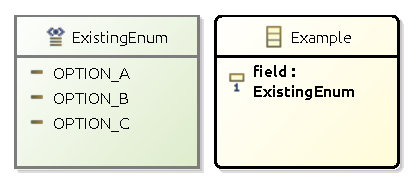
\includegraphics{images/05_library_of_transformations/02_type_level_transformations/07_enum_fields/enum_field.pdf}
        \caption{$Tm_{EnumField}$ for $.\type{ExistingEnum}$ \\with $name = \type{field}$}
        \label{fig:library_of_transformations:type_level_transformations:enum_fields:visualisation:ecore}
    \end{subfigure}
    \begin{subfigure}{0.45\textwidth}
        \centering
        % To use this figure in your LaTeX document
% import the package groove/resources/groove2tikz.sty
%
\begin{tikzpicture}[scale=\tikzscale,name prefix=test-]
\node[type_node] (n0) at (3.125, -0.945) {\ml{\textbf{Example}}};
\node[type_node] (n2) at (5.570, -0.970) {\ml{\textbf{ExistingEnum}\\\textit{OPTION\_A}\\\textit{OPTION\_B}\\\textit{OPTION\_C}}};

\path[basic_edge](n0.east |- 5.570, -0.970) -- node[lab] {\ml{field}} (n2) ;
\end{tikzpicture}

        \caption{$TG_{EnumFieldFlags}$ for $\type{ExistingEnum}$ \\with $name = \type{field}$}
        \label{fig:library_of_transformations:type_level_transformations:enum_fields:visualisation:groove_flags}
    \end{subfigure}
    \\
    \begin{subfigure}{0.95\textwidth}
        \centering
        % To use this figure in your LaTeX document
% import the package groove/resources/groove2tikz.sty
%
\begin{tikzpicture}[scale=\tikzscale,name prefix=test-]
\node[type_node] (n0) at (3.125, -0.945) {\ml{\textbf{Example}}};
\node[type_node] (n2) at (5.570, -0.970) {\ml{\textit{\textbf{ExistingEnum}}}};
\node[type_node] (n3) at (2.970, -0.170) {\ml{\textbf{ExistingEnum\$OPTION\_A}}};
\node[type_node] (n4) at (5.570, -0.170) {\ml{\textbf{ExistingEnum\$OPTION\_B}}};
\node[type_node] (n5) at (8.170, -0.170) {\ml{\textbf{ExistingEnum\$OPTION\_C}}};

\path[subtype_edge] (n3)  --  (n2) ;
\path[subtype_edge](n4.south -| 5.570, -0.970) --  (n2) ;
\path[subtype_edge] (n5)  --  (n2) ;
\path[basic_edge](n0.east |- 5.570, -0.970) -- node[lab] {\ml{field}} (n2) ;
\end{tikzpicture}

        \caption{$TG_{EnumFieldNodes}$ for $\type{ExistingEnum}$ with $name = \type{field}$}
        \label{fig:library_of_transformations:type_level_transformations:enum_fields:visualisation:groove_nodes}
    \end{subfigure}
    \caption{Visualisation of the transformation of a field typed by an enumeration type}
    \label{fig:library_of_transformations:type_level_transformations:enum_fields:visualisation}
\end{figure}

In this section, the transformation for a field typed by an enumeration type will be discussed. Since an enumeration type can be encoded in multiple ways, multiple encodings will be introduced for fields as well. First, the Ecore type model will be introduced.

\begin{defin}[Type model $Tm_{EnumField}$]
\label{defin:library_of_transformations:type_level_transformations:enum_fields:tmod_enum_field}
Let $Tm_{EnumField}$ be the type model containing a regular class with identifier $classtype$. Furthermore, it defines an enumeration type with identifier $enumid$, and corresponding values as set $enumvalues$. Then $Tm_{EnumField}$ defines a field named $name$ with type $enumid$ on class $classtype$. $Tm_{EnumField}$ is defined as:
\begin{align*}
Class =\ &\{classtype\} \\
Enum =\ &\{enumid\} \\
UserDataType =\ &\{\} \\
Field =\ &\{(classtype, name)\} \\
\mathrm{FieldSig} =\ &\begin{cases}
    (f, (enumid, 1..1)) &\mathrm{if}\ f \in Field_{Tm_{EnumField}}
\end{cases} \\
EnumValue =\ &\{(enumid, v) \mid v \in enumvalues\} \\
Inh =\ &\{\} \\
Prop =\ &\{\} \\
Constant =\ &\{\} \\
\mathrm{ConstType} =\ &\{\}
\end{align*}
\isabellelref{tmod_enum_field}{Ecore-GROOVE-Mapping-Library.EnumField}
\end{defin}

\begin{thm}[Correctness of $Tm_{EnumField}$]
\label{defin:library_of_transformations:type_level_transformations:enum_fields:tmod_enum_field_correct}
$Tm_{EnumField}$ (\cref{defin:library_of_transformations:type_level_transformations:enum_fields:tmod_enum_field}) is a consistent type model in the sense of \cref{defin:formalisations:ecore_formalisation:type_models:type_model_consistency}.
\isabellelref{tmod_enum_field_correct}{Ecore-GROOVE-Mapping-Library.EnumField}
\end{thm}

A visual representation of $Tm_{EnumField}$ with field name $\type{field}$ on class $.\type{Example}$ can be seen in \cref{fig:library_of_transformations:type_level_transformations:enum_fields:visualisation:ecore}. In this example, the field is typed by the $.\type{ExistingEnum}$ enumeration type. The correctness proof of $Tm_{EnumField}$ is more involved, it is not included here for conciseness. It can be found within the validated Isabelle proofs.

In order to make composing transformation functions possible, $Tm_{EnumField}$ should be compatible with the type model it is combined with.

\begin{thm}[Correctness of $\mathrm{combine}(Tm, Tm_{EnumField})$]
\label{defin:library_of_transformations:type_level_transformations:enum_fields:tmod_enum_field_combine_correct}
Assume a type model $Tm$ that is consistent in the sense of \cref{defin:formalisations:ecore_formalisation:type_models:type_model_consistency}. Then $Tm$ is compatible with $Tm_{EnumField}$ (in the sense of \cref{defin:transformation_framework:type_models_and_type_graphs:combining_type_models:compatibility}) if:
\begin{itemize}
    \item The class type on which the field is defined, $classtype$, is already an existing class in $Tm$;
    \item The enumeration type by which the field is typed, $enumid$, is already an existing enumeration type in $Tm$;
    \item All the values for the enumeration type $enumid$ are already enumeration values for $enumid$ in $Tm$;
    \item The field named $name$ is not already a field on $classtype$ in $Tm$.
\end{itemize}
\isabellelref{tmod_enum_field_combine_correct}{Ecore-GROOVE-Mapping-Library.EnumField}
\end{thm}

\begin{proof}
Use \cref{defin:transformation_framework:type_models_and_type_graphs:combining_type_models:tmod_combine_merge_correct}. It is possible to show that all assumptions hold. Now we have shown that $\mathrm{combine}(Tm, Tm_{EnumField})$ is consistent in the sense of \cref{defin:formalisations:ecore_formalisation:type_models:type_model_consistency}.
\end{proof}

The definitions and theorems for defining a field typed by an enumeration type within Ecore are now complete. 

\subsubsection{Encoding as edge type to an node type encoded enumeration type}

As mentioned earlier, \cref{subsec:library_of_transformations:type_level_transformations:enumeration_types} defines multiple ways to encode an enumeration type. Each of these encodings needs a specialised field encoding. In principle, the encoding of the fields itself is the same, but since every transformation model needs to be valid on its own, the encodings need to be distinguished. 

The first encoding for an enumeration type uses node types to encode the different values. The encoding corresponding to $Tm_{EnumField}$, in the case that the field references an enumeration type encoded as node types, can then be represented as $TG_{EnumFieldNodes}$, defined in the following definition:

\begin{defin}[Type graph $TG_{EnumFieldNodes}$]
\label{defin:library_of_transformations:type_level_transformations:enum_fields:tg_enum_as_node_types_field_as_edge_type}
Let $TG_{EnumFieldNodes}$ be the type graph containing a node type which encodes the class type $classtype$.
Furthermore, $TG_{EnumFieldNodes}$ contains an encoded version of enumeration type $enumid$ with values from set $enumvalues$. This enumeration type is encoded using node types, as defined in $TG_{EnumNodes}$ (\cref{defin:library_of_transformations:type_level_transformations:enumeration_types:tg_enum_as_node_types}). Finally, $TG_{EnumFieldNodes}$ defines an edge type from the encoded $classtype$ named $name$ to the encoded enumeration type $enumid$. $TG_{EnumFieldNodes}$ is defined as:
\begin{align*}
NT =\ &\{\mathrm{ns\_\!to\_\!list}(classtype), \mathrm{ns\_\!to\_\!list}(enumid)\}\ \cup \\&\{ \mathrm{ns\_\!to\_\!list}(enumid) \append \langle v \rangle \mid v \in enumvalues \}\\
ET =\ &\{(\mathrm{ns\_\!to\_\!list}(classtype), \langle name \rangle, \mathrm{ns\_\!to\_\!list}(enumid))\} \\
\!\!\sqsubseteq\ =\ &\{(\mathrm{ns\_\!to\_\!list}(classtype), \mathrm{ns\_\!to\_\!list}(classtype)),\ \\& (\mathrm{ns\_\!to\_\!list}(enumid), \mathrm{ns\_\!to\_\!list}(enumid))\}\ \cup \\&
\{(\mathrm{ns\_\!to\_\!list}(enumid) \append \langle v \rangle, \mathrm{ns\_\!to\_\!list}(enumid) \append \langle v \rangle) \mid v \in enumvalues \}\ \cup \\&
\{(\mathrm{ns\_\!to\_\!list}(enumid) \append \langle v \rangle, \mathrm{ns\_\!to\_\!list}(enumid)) \mid v \in enumvalues \} \\
abs =\ &\{\mathrm{ns\_\!to\_\!list}(enumid)\} \\
\mathrm{mult}(e) =\ &\begin{cases}
    (0..\mstar, 1..1) &\mathrm{if}\ e \in \{(\mathrm{ns\_\!to\_\!list}(classtype), \langle name \rangle, \mathrm{ns\_\!to\_\!list}(enumid))\}
\end{cases} \\
contains =\ &\{\}
\end{align*}
\isabellelref{tg_enum_as_node_types_field_as_edge_type}{Ecore-GROOVE-Mapping-Library.EnumField}
\end{defin}

\begin{thm}[Correctness of $TG_{EnumFieldNodes}$]
\label{defin:library_of_transformations:type_level_transformations:enum_fields:tg_enum_as_node_types_field_as_edge_type_correct}
$TG_{EnumFieldNodes}$ (\cref{defin:library_of_transformations:type_level_transformations:enum_fields:tg_enum_as_node_types_field_as_edge_type}) is a valid type graph in the sense of \cref{defin:formalisations:groove_formalisation:type_graphs:type_graph_validity}.
\isabellelref{tg_enum_as_node_types_field_as_edge_type_correct}{Ecore-GROOVE-Mapping-Library.EnumField}
\end{thm}

A visual representation of $TG_{EnumFieldNodes}$ with edge name $\type{field}$ on node type $\type{Example}$ can be seen in \cref{fig:library_of_transformations:type_level_transformations:enum_fields:visualisation:groove_nodes}. The field references the encoded enumeration type $\type{ExistingEnum}$ via the abstract type, such that its nodes can reference any of the concrete values. The correctness proof of $TG_{EnumFieldNodes}$ is more involved, it is not included here for conciseness. It can be found within the validated Isabelle proofs.

In order to make composing transformation functions possible, $TG_{EnumFieldNodes}$ should be compatible with the type graph it is combined with.

\begin{thm}[Correctness of $\mathrm{combine}(TG, TG_{EnumFieldNodes})$]
\label{defin:library_of_transformations:type_level_transformations:enum_fields:tg_enum_as_node_types_field_as_edge_type_combine_correct}
Assume a type graph $TG$ that is valid in the sense of \cref{defin:formalisations:groove_formalisation:type_graphs:type_graph_validity}. Then $TG$ is compatible with $TG_{EnumFieldNodes}$ (in the sense of \cref{defin:transformation_framework:type_models_and_type_graphs:combining_type_graphs:compatibility}) if:
\begin{itemize}
    \item The node type of the encoded class type in $TG_{EnumFieldNodes}$ is already an node type in $TG$;
    \item All node types corresponding to the encoding of the enumeration type in $TG_{EnumFieldNodes}$ are already node types in $TG$;
    \item The node type of the encoded class type in $TG_{EnumFieldNodes}$ does not already have an edge type with the same name as the field in $TG$.
\end{itemize}
\isabellelref{tg_enum_as_node_types_field_as_edge_type_combine_correct}{Ecore-GROOVE-Mapping-Library.EnumField}
\end{thm}

\begin{proof}
Use \cref{defin:transformation_framework:type_models_and_type_graphs:combining_type_graphs:tg_combine_merge_correct}. It is possible to show that all assumptions hold. Now we have shown that $\mathrm{combine}(TG, TG_{EnumFieldNodes})$ is valid in the sense of \cref{defin:formalisations:groove_formalisation:type_graphs:type_graph_validity}.
\end{proof}

The next definitions define the transformation function from $Tm_{EnumField}$ to $TG_{EnumFieldNodes}$:

\begin{defin}[Transformation function $f_{EnumFieldNodes}$]
\label{defin:library_of_transformations:type_level_transformations:enum_fields:tmod_enum_field_to_tg_enum_as_node_types_field_as_edge_type}
The transformation function $f_{EnumFieldNodes}(Tm)$ is defined as:
\begin{align*}
NT =\ &\{\mathrm{ns\_\!to\_\!list}(t) \mid t \in Class_{Tm} \cup Enum_{Tm}\}\ \cup \\&\{ \mathrm{ns\_\!to\_\!list}(e) \append \langle v \rangle \mid (e, v) \in EnumValue_{Tm} \}\\
ET =\ &\{(\mathrm{ns\_\!to\_\!list}(c), \langle f \rangle, \mathrm{ns\_\!to\_\!list}(e)) \mid (c, f) \in Field_{Tm} \land e \in Enum_{Tm}\} \\
\!\!\sqsubseteq\ =\ &\{(\mathrm{ns\_\!to\_\!list}(x), \mathrm{ns\_\!to\_\!list}(x)) \mid x \in Class_{Tm} \cup Enum_{Tm} \}\ \cup \\&
\{(\mathrm{ns\_\!to\_\!list}(e) \append \langle v \rangle, \mathrm{ns\_\!to\_\!list}(e) \append \langle v \rangle) \mid (e, v) \in EnumValue_{Tm} \}\ \cup \\&
\{(\mathrm{ns\_\!to\_\!list}(e) \append \langle v \rangle, \mathrm{ns\_\!to\_\!list}(e)) \mid (e, v) \in EnumValue_{Tm} \} \\
abs =\ &\{\mathrm{ns\_\!to\_\!list}(t) \mid t \in Enum_{Tm}\}\ \\
\mathrm{mult}(e) =\ &\begin{cases}
    (0..\mstar, 1..1) &\mathrm{if}\ e \in \{(\mathrm{ns\_\!to\_\!list}(c), \langle f \rangle, \mathrm{ns\_\!to\_\!list}(e)) \mid (c, f) \in Field_{Tm} \land e \in Enum_{Tm}\}
\end{cases} \\
contains =\ &\{\}
\end{align*}
\isabellelref{tmod_enum_field_to_tg_enum_as_node_types_field_as_edge_type}{Ecore-GROOVE-Mapping-Library.EnumField}
\end{defin}

\begin{thm}[Correctness of $f_{EnumFieldNodes}$]
\label{defin:library_of_transformations:type_level_transformations:enum_fields:tmod_enum_field_to_tg_enum_as_node_types_field_as_edge_type_func}
$f_{EnumFieldNodes}(Tm)$ (\cref{defin:library_of_transformations:type_level_transformations:enum_fields:tmod_enum_field_to_tg_enum_as_node_types_field_as_edge_type}) is a valid transformation function in the sense of \cref{defin:transformation_framework:type_models_and_type_graphs:combining_transformation_functions:transformation_function_type_model_type_graph} transforming $Tm_{EnumField}$ into $TG_{EnumFieldNodes}$.
\isabellelref{tmod_enum_field_to_tg_enum_as_node_types_field_as_edge_type_func}{Ecore-GROOVE-Mapping-Library.EnumField}
\end{thm}

The proof of the correctness of $f_{EnumFieldNodes}$ will not be included here. Instead, it can be found in the validated Isabelle theories.

Finally, to complete the transformation, the transformation function that transforms $TG_{EnumFieldNodes}$ into $Tm_{EnumField}$ is defined:

\begin{defin}[Transformation function $f'_{EnumFieldNodes}$]
\label{defin:library_of_transformations:type_level_transformations:enum_fields:tg_enum_as_node_types_field_as_edge_type_to_tmod_enum_field}
The transformation function $f'_{EnumFieldNodes}(TG)$ is defined as:
\begin{align*}
Class =\ &\{\mathrm{list\_\!to\_\!ns}(n) \mid n \in NT_{TG} \land n = \mathrm{ns\_\!to\_\!list}(classtype) \} \\
Enum =\ &\{\mathrm{list\_\!to\_\!ns}(n) \mid n \in NT_{TG} \land n = \mathrm{ns\_\!to\_\!list}(enumid) \} \\
UserDataType =\ &\{\} \\
Field =\ &\{(\mathrm{list\_\!to\_\!ns}(\mathrm{src}(e)), l) \mid e \in ET_{TG} \land \langle l \rangle = \mathrm{lab}(e) \} \\
\mathrm{FieldSig} =\ &\begin{cases}
    (f, (fieldtype, 1..1)) &\mathrm{if}\ f \in \{(\mathrm{list\_\!to\_\!ns}(\mathrm{src}(e)), l) \mid e \in ET_{TG} \land \langle l \rangle = \mathrm{lab}(e) \}
\end{cases} \\
EnumValue =\ &\{(enumid, v) \mid v \in enumvalues\} \\
Inh =\ &\{\} \\
Prop =\ &\{\} \\
Constant =\ &\{\} \\
\mathrm{ConstType} =\ &\{\}
\end{align*}
\isabellelref{tg_enum_as_node_types_field_as_edge_type_to_tmod_enum_field}{Ecore-GROOVE-Mapping-Library.EnumField}
\end{defin}

\begin{thm}[Correctness of $f'_{EnumFieldNodes}$]
\label{defin:library_of_transformations:type_level_transformations:enum_fields:tg_enum_as_node_types_field_as_edge_type_to_tmod_enum_field_func}
$f'_{EnumFieldNodes}(TG)$ (\cref{defin:library_of_transformations:type_level_transformations:enum_fields:tg_enum_as_node_types_field_as_edge_type_to_tmod_enum_field}) is a valid transformation function in the sense of \cref{defin:transformation_framework:type_models_and_type_graphs:combining_transformation_functions:transformation_function_type_graph_type_model} transforming $TG_{EnumFieldNodes}$ into $Tm_{EnumField}$.
\isabellelref{tg_enum_as_node_types_field_as_edge_type_to_tmod_enum_field_func}{Ecore-GROOVE-Mapping-Library.EnumField}
\end{thm}

Once more, the correctness proof is not included here but can be found in the validated Isabelle proofs of this thesis.

\subsubsection{Encoding as edge type to an flag encoded enumeration type}

The second encoding for an enumeration type uses flags to encode the different values. The encoding corresponding to $Tm_{EnumField}$, in the case that the field references an enumeration type encoded as flags, can then be represented as $TG_{EnumFieldFlags}$, defined in the following definition:

\begin{defin}[Type graph $TG_{EnumFieldFlags}$]
\label{defin:library_of_transformations:type_level_transformations:enum_fields:tg_enum_as_flags_field_as_edge_type}
Let $TG_{EnumFieldFlags}$ be the type graph containing a node type which encodes the class type $classtype$.
Furthermore, $TG_{EnumFieldFlags}$ contains an encoded version of enumeration type $enumid$ with values from set $enumvalues$. This enumeration type is encoded using flags, as defined in $TG_{EnumFlags}$ (\cref{defin:library_of_transformations:type_level_transformations:enumeration_types:tg_enum_as_flags}). Finally, $TG_{EnumFieldFlags}$ defines an edge type from the encoded $classtype$ named $name$ to the encoded enumeration type $enumid$. $TG_{EnumFieldFlags}$ is defined as:
\begin{align*}
NT =\ &\{\mathrm{ns\_\!to\_\!list}(classtype), \mathrm{ns\_\!to\_\!list}(enumid)\}\\
ET =\ &\{(\mathrm{ns\_\!to\_\!list}(classtype), \langle name \rangle, \mathrm{ns\_\!to\_\!list}(enumid))\}\\
\!\!\sqsubseteq\ =\ &\{(\mathrm{ns\_\!to\_\!list}(classtype), \mathrm{ns\_\!to\_\!list}(classtype)),\ \\& (\mathrm{ns\_\!to\_\!list}(enumid), \mathrm{ns\_\!to\_\!list}(enumid))\}\\
abs =\ &\{\} \\
\mathrm{mult}(e) =\ &\begin{cases}
    (0..\mstar, 1..1) &\mathrm{if}\ e \in \{(\mathrm{ns\_\!to\_\!list}(classtype), \langle name \rangle, \mathrm{ns\_\!to\_\!list}(enumid))\}
\end{cases} \\
contains =\ &\{\}
\end{align*}
\isabellelref{tg_enum_as_flags_field_as_edge_type}{Ecore-GROOVE-Mapping-Library.EnumField}
\end{defin}

\begin{thm}[Correctness of $TG_{EnumFieldFlags}$]
\label{defin:library_of_transformations:type_level_transformations:enum_fields:tg_enum_as_flags_field_as_edge_type_correct}
$TG_{EnumFieldFlags}$ (\cref{defin:library_of_transformations:type_level_transformations:enum_fields:tg_enum_as_flags_field_as_edge_type}) is a valid type graph in the sense of \cref{defin:formalisations:groove_formalisation:type_graphs:type_graph_validity}.
\isabellelref{tg_enum_as_flags_field_as_edge_type_correct}{Ecore-GROOVE-Mapping-Library.EnumField}
\end{thm}

A visual representation of $TG_{EnumFieldFlags}$ with edge name $\type{field}$ on node type $\type{Example}$ can be seen in \cref{fig:library_of_transformations:type_level_transformations:enum_fields:visualisation:groove_flags}. The field references the encoded enumeration type $\type{ExistingEnum}$ via the corresponding node type. The correctness proof of $TG_{EnumFieldFlags}$ is more involved, it is not included here for conciseness. It can be found within the validated Isabelle proofs.

In order to make composing transformation functions possible, $TG_{EnumFieldFlags}$ should be compatible with the type graph it is combined with.

\begin{thm}[Correctness of $\mathrm{combine}(TG, TG_{EnumFieldFlags})$]
\label{defin:library_of_transformations:type_level_transformations:enum_fields:tg_enum_as_flags_field_as_edge_type_combine_correct}
Assume a type graph $TG$ that is valid in the sense of \cref{defin:formalisations:groove_formalisation:type_graphs:type_graph_validity}. Then $TG$ is compatible with $TG_{EnumFieldFlags}$ (in the sense of \cref{defin:transformation_framework:type_models_and_type_graphs:combining_type_graphs:compatibility}) if:
\begin{itemize}
    \item The node type of the encoded class type in $TG_{EnumFieldFlags}$ is already an node type in $TG$;
    \item All node types corresponding to the encoding of the enumeration type in $TG_{EnumFieldFlags}$ are already node types in $TG$;
    \item The node type of the encoded class type in $TG_{EnumFieldFlags}$ does not already have an edge type with the same name as the field in $TG$.
\end{itemize}
\isabellelref{tg_enum_as_flags_field_as_edge_type_combine_correct}{Ecore-GROOVE-Mapping-Library.EnumField}
\end{thm}

\begin{proof}
Use \cref{defin:transformation_framework:type_models_and_type_graphs:combining_type_graphs:tg_combine_merge_correct}. It is possible to show that all assumptions hold. Now we have shown that $\mathrm{combine}(TG, TG_{EnumFieldFlags})$ is valid in the sense of \cref{defin:formalisations:groove_formalisation:type_graphs:type_graph_validity}.
\end{proof}

The next definitions define the transformation function from $Tm_{EnumField}$ to $TG_{EnumFieldFlags}$:

\begin{defin}[Transformation function $f_{EnumFieldFlags}$]
\label{defin:library_of_transformations:type_level_transformations:enum_fields:tmod_enum_field_to_tg_enum_as_flags_field_as_edge_type}
The transformation function $f_{EnumFieldFlags}(Tm)$ is defined as:
\begin{align*}
NT =\ &\{\mathrm{ns\_\!to\_\!list}(t) \mid t \in Class_{Tm} \cup Enum_{Tm}\}\\
ET =\ &\{(\mathrm{ns\_\!to\_\!list}(c), \langle f \rangle, \mathrm{ns\_\!to\_\!list}(e)) \mid (c, f) \in Field_{Tm} \land e \in Enum_{Tm}\} \\
\!\!\sqsubseteq\ =\ &\{(\mathrm{ns\_\!to\_\!list}(x), \mathrm{ns\_\!to\_\!list}(x)) \mid x \in Class_{Tm} \cup Enum_{Tm} \}\\
abs =\ &\{\}\ \\
\mathrm{mult}(e) =\ &\begin{cases}
    (0..\mstar, 1..1) &\mathrm{if}\ e \in \{(\mathrm{ns\_\!to\_\!list}(c), \langle f \rangle, \mathrm{ns\_\!to\_\!list}(e)) \mid (c, f) \in Field_{Tm} \land e \in Enum_{Tm}\}
\end{cases} \\
contains =\ &\{\}
\end{align*}
\isabellelref{tmod_enum_field_to_tg_enum_as_flags_field_as_edge_type}{Ecore-GROOVE-Mapping-Library.EnumField}
\end{defin}

\begin{thm}[Correctness of $f_{EnumFieldFlags}$]
\label{defin:library_of_transformations:type_level_transformations:enum_fields:tmod_enum_field_to_tg_enum_as_flags_field_as_edge_type_func}
$f_{EnumFieldFlags}(Tm)$ (\cref{defin:library_of_transformations:type_level_transformations:enum_fields:tmod_enum_field_to_tg_enum_as_flags_field_as_edge_type}) is a valid transformation function in the sense of \cref{defin:transformation_framework:type_models_and_type_graphs:combining_transformation_functions:transformation_function_type_model_type_graph} transforming $Tm_{EnumField}$ into $TG_{EnumFieldFlags}$.
\isabellelref{tmod_enum_field_to_tg_enum_as_flags_field_as_edge_type_func}{Ecore-GROOVE-Mapping-Library.EnumField}
\end{thm}

The proof of the correctness of $f_{EnumFieldFlags}$ will not be included here. Instead, it can be found in the validated Isabelle theories.

Finally, to complete the transformation, the transformation function that transforms $TG_{EnumFieldFlags}$ into $Tm_{EnumField}$ is defined:

\begin{defin}[Transformation function $f'_{EnumFieldFlags}$]
\label{defin:library_of_transformations:type_level_transformations:enum_fields:tg_enum_as_flags_field_as_edge_type_to_tmod_enum_field}
The transformation function $f'_{EnumFieldFlags}(TG)$ is defined as:
\begin{align*}
Class =\ &\{\mathrm{list\_\!to\_\!ns}(n) \mid n \in NT_{TG} \land n = \mathrm{ns\_\!to\_\!list}(classtype) \} \\
Enum =\ &\{\mathrm{list\_\!to\_\!ns}(n) \mid n \in NT_{TG} \land n = \mathrm{ns\_\!to\_\!list}(enumid) \} \\
UserDataType =\ &\{\} \\
Field =\ &\{(\mathrm{list\_\!to\_\!ns}(\mathrm{src}(e)), l) \mid e \in ET_{TG} \land \langle l \rangle = \mathrm{lab}(e) \} \\
\mathrm{FieldSig} =\ &\begin{cases}
    (f, (fieldtype, 1..1)) &\mathrm{if}\ f \in \{(\mathrm{list\_\!to\_\!ns}(\mathrm{src}(e)), l) \mid e \in ET_{TG} \land \langle l \rangle = \mathrm{lab}(e) \}
\end{cases} \\
EnumValue =\ &\{(enumid, v) \mid v \in enumvalues\} \\
Inh =\ &\{\} \\
Prop =\ &\{\} \\
Constant =\ &\{\} \\
\mathrm{ConstType} =\ &\{\}
\end{align*}
\isabellelref{tg_enum_as_flags_field_as_edge_type_to_tmod_enum_field}{Ecore-GROOVE-Mapping-Library.EnumField}
\end{defin}

\begin{thm}[Correctness of $f'_{EnumFieldFlags}$]
\label{defin:library_of_transformations:type_level_transformations:enum_fields:tg_enum_as_flags_field_as_edge_type_to_tmod_enum_field_func}
$f'_{EnumFieldFlags}(TG)$ (\cref{defin:library_of_transformations:type_level_transformations:enum_fields:tg_enum_as_flags_field_as_edge_type_to_tmod_enum_field}) is a valid transformation function in the sense of \cref{defin:transformation_framework:type_models_and_type_graphs:combining_transformation_functions:transformation_function_type_graph_type_model} transforming $TG_{EnumFieldFlags}$ into $Tm_{EnumField}$.
\isabellelref{tg_enum_as_flags_field_as_edge_type_to_tmod_enum_field_func}{Ecore-GROOVE-Mapping-Library.EnumField}
\end{thm}

Once more, the correctness proof is not included here but can be found in the validated Isabelle proofs of this thesis.